
\subsection{Evaluation of CVMs through Validation}

One key aspect in earthquake ground motion simulation is the validation of synthetic seismograms against data recorded during past earthquakes. This helps test both models and simulation methods. A particular event of relevance is the 29 July 2008 \eqmag{w} 5.4 Chino Hills earthquake in southern California. This moderate earthquake, the strongest in the Los Angeles area since the 1994 Northridge earthquake, caused no significant damage or fatalities, but provided an excellent opportunity for earthquake research because it was recorded by over 500 seismic monitoring stations in California and other neighboring states. 

Various recent studies have included simulations of the 2008 Chino Hills earthquake with models created using the UCVM mesh generation utilities \citep[e.g.,][]{Olsen_2010_SRL, Taborda_2013_BSSA, Taborda_2014_BSSA}. These simulations have helped test current modeling approaches to predict the ground motion of moderate magnitude earthquakes at low ($<1$~Hz), medium (1--4~Hz), and high ($>4$~Hz) frequencies using deterministic and hybrid methods. They have as well as provided a context to propose and test different validation algorithms (goodness-of-fit criteria). More important, in the context of using UCVM, these simulations have helped evaluate the various CVMs available for the southern California region, and how their differences impact simulation results used for engineering applications.

\citet{Taborda_2014_BSSA}, in particular, focuses on the validation of simulations of the Chino Hills earthquake using different velocity models, namely CVM-S and CVM-H. The discrete representations of these models used as input for their simulations were created using UCVM meshing programs. The authors evaluate the differences between these two models and their effect on validation results through comparisons with recorded seismograms from over 300 stations scattered throughout a simulation-domain area of \adomain{180}{135}{km}. Figure \ref{fig:ch.validation} shows comparisons between the surface \vs{} from the two models, the simulation outcome for peak ground velocity, the results of a goodness-of-fit validation analysis, and the differences of attenuation relationships derived fromt he simulations with respect to the data attenuation and empirical relationships typically used in engineering applications. Here, we highlight that the discrete input models used in these simulations were created utilizing the etree MPI utilities of UCVM and built on Kraken (now decommissioned) at the National Institute for Computational Sciences and on NCSA's Blue Waters supercomputer systems. The etree databases ranged between 110 and 260 GB, and the resulting finite-element models comprised meshes ranging between 5 billion and 15 billion octants.


% ---------------------------------------------------------------------------------------------
% TEMP FIGURE: Needs to be improved in Illustrator and moved to final PDF dir.
\begin{figure*}[ht!]
	\centering
	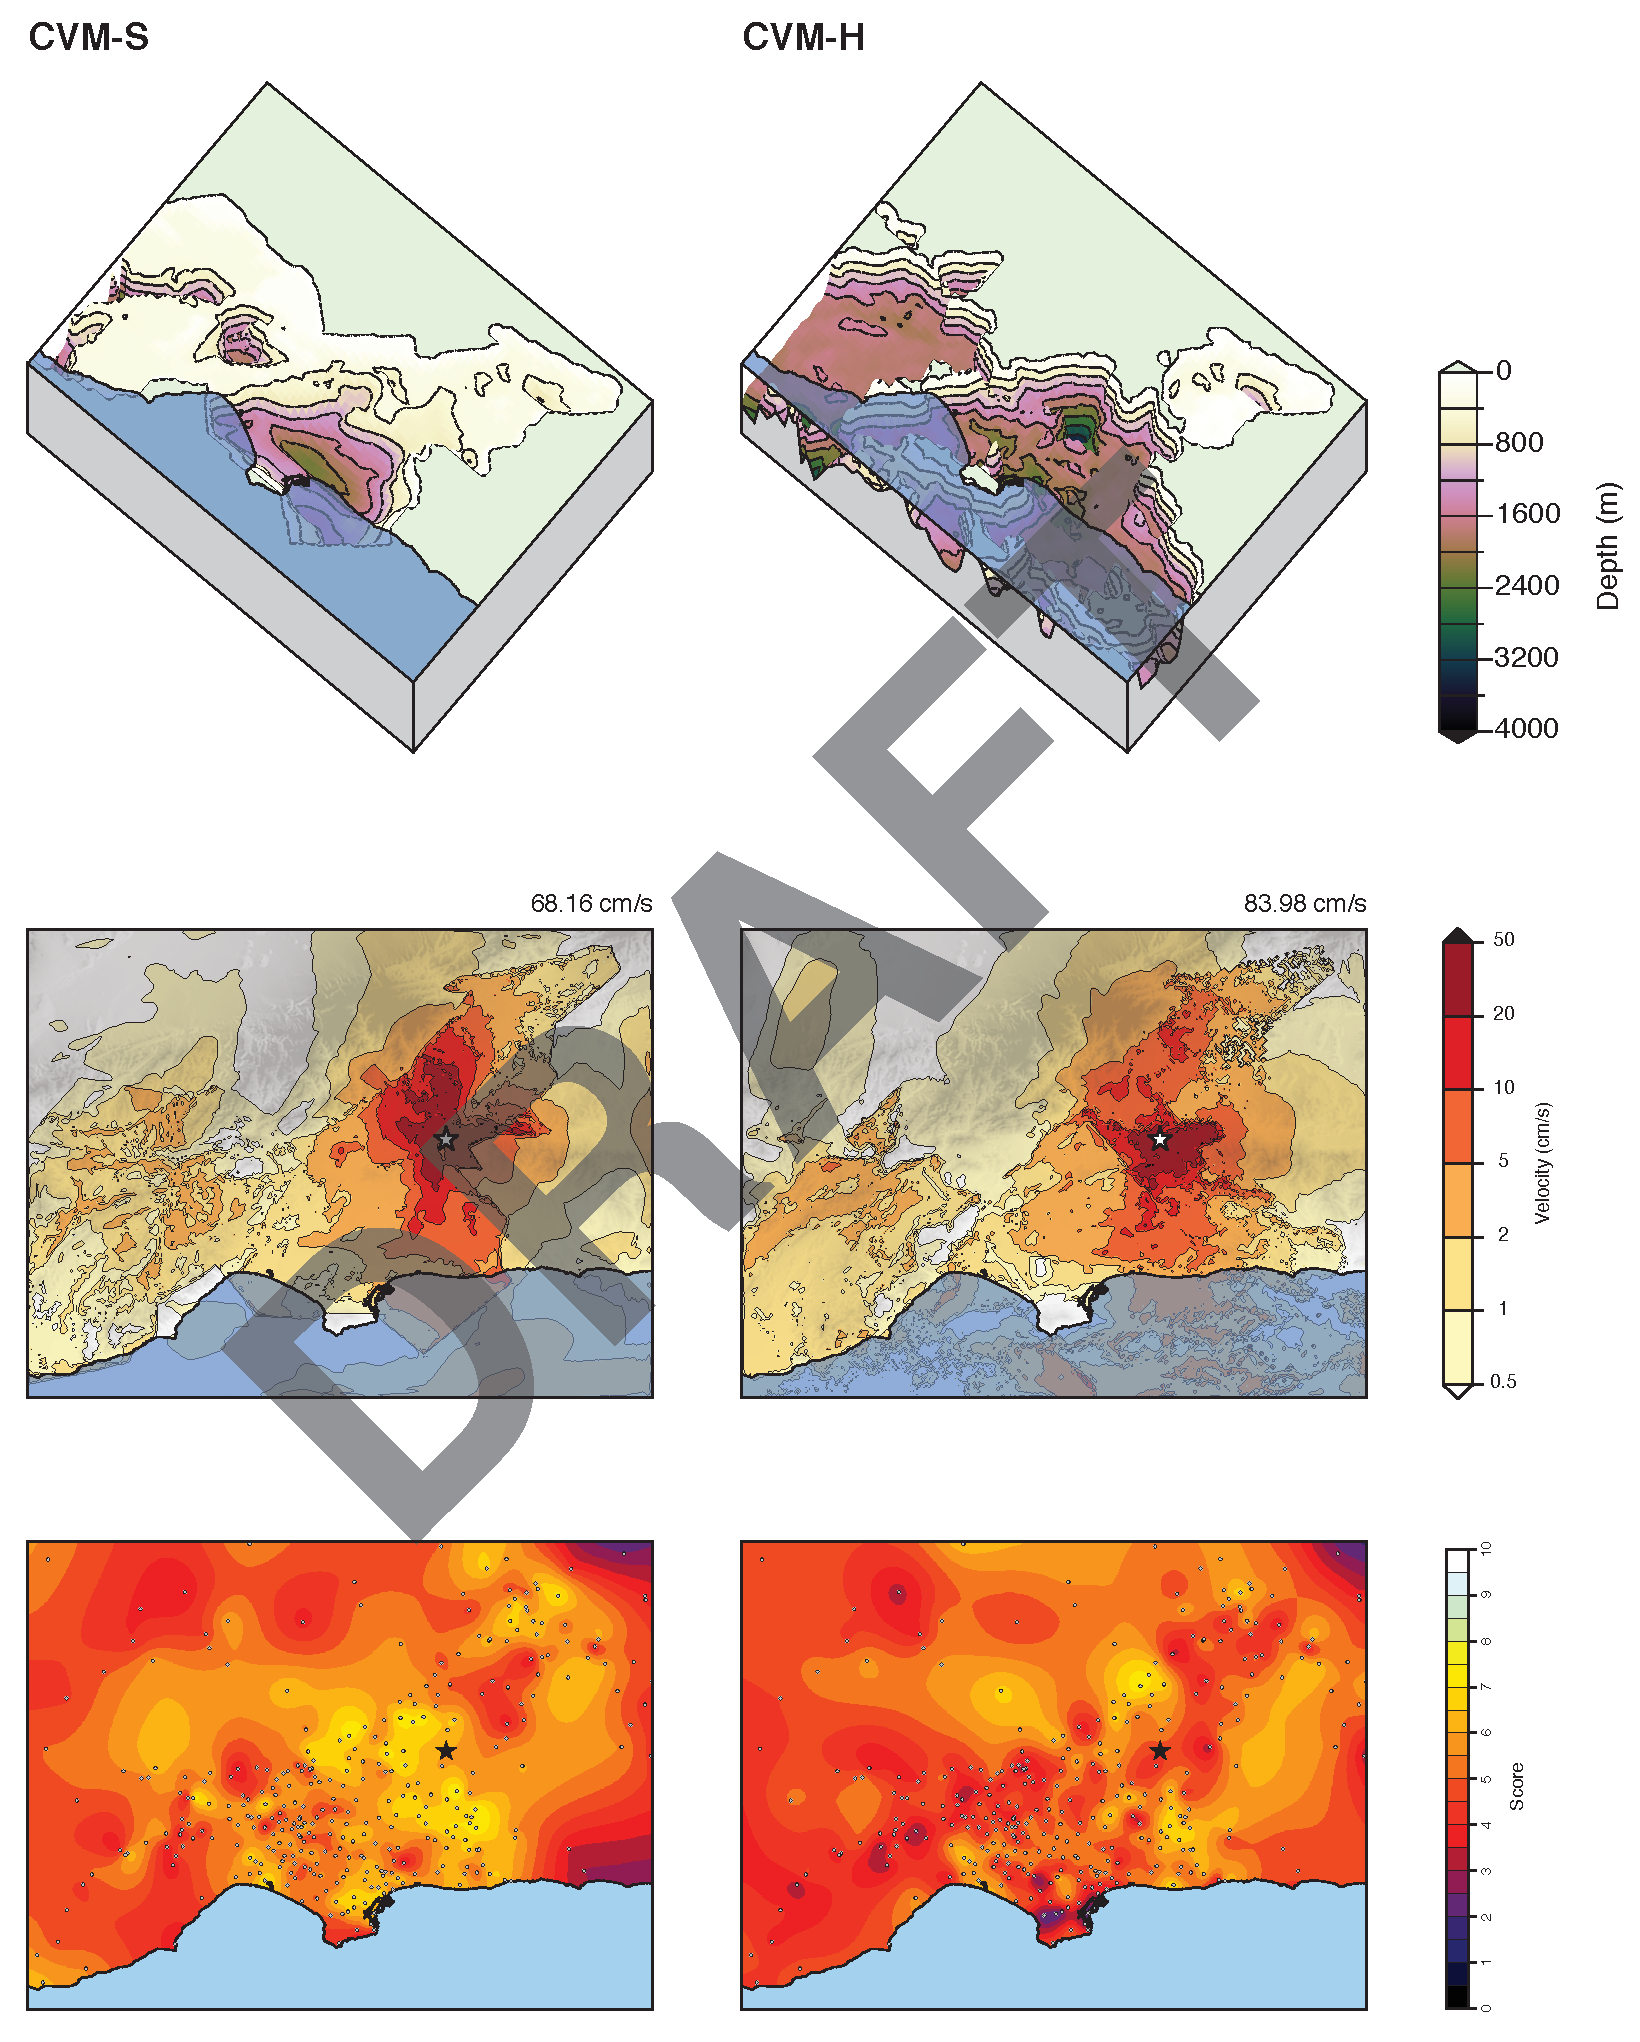
\includegraphics
		[width=0.75\textwidth]
		{figures/raw-pdf/ch-validation}
	\caption{\textcolor{red}{Temporary mock-up figure showing results from Chino Hills validation.}}
	\label{fig:ch.validation}
\end{figure*}
% ---------------------------------------------------------------------------------------------


% OLD TEXT
% ********

%\subsection{The 2008 Chino Hills Case Study}
%
%On 29 July 2008 at 11:42 a.m. a magnitude \eqmag{w} 5.4 earthquake occurred in southern California. Dubbed the Chino Hills earthquake, it was the strongest felt in the city since the 1994 Northridge earthquake, but caused no significant damage or fatalities. It provided, nonetheless, an excellent opportunity for earthquake studies because its shaking was recorded on a numerous set of monitoring stations. Since then, UCVM and other SCEC initiatives have used the data gathered during this earthquake as a case study for testing different simulation methods and models. 
%
%Various recent studies have carefully conducted validations of simulations of the 2008 Chino Hills earthquake with models created using UCVM \citep[e.g.,][]{Olsen_2010_SRL, Taborda_2013_BSSA, Taborda_2014_BSSA}. They have helped test the simulation capabilities of current modeling approaches to predict the ground motion of moderate magnitude earthquakes at low ($<1$~Hz), moderate (1--4~Hz), and high ($>4$~Hz) frequencies using deterministic and hybrid methods, as well as provide a context to propose and test different validation algorithms (goodness-of-fit criteria). 
%
%The latest of these studies \citep{Taborda_2014_BSSA} focuses on the validation of simulations of the Chino Hills earthquake using the CVM-S and CVM-H velocity models. This in turn has helped evaluate the differences between the models and model accuracy. The validation performed in this study is based on comparisons with recorded seismograms in over 300 stations scattered throughout the region. The simulation and the models created with UCVM cover an area of \adomain{180}{135}{km} and go as deep as 62~km. Figure \ref{fig:ch.validation} shows comparisons between the crustal structures of the two models, results of the surface peak ground velocity obtained from the simulations and contour maps of the validation results. The models created for these simulations were built using the etree MPI utilities on NICS's Kraken and NCSA's Blue Waters supercomputer systems employing between XX and YY thousand cores for up to ZZ hours. The sizes of the output (etree) files range between XXX and XXX GB and they comprised between 5 billion and 15 billion octants. \textcolor{red}{(This paragraph needs to be improved.)}

%\textcolor{green}{Do the logfiles still exist? Can provide runtimes, resources used (core hours, wallclock), and where it was run.}

% ********
